% =====================================================================
%  Online PAC Labeling from a Linear Programming Perspective
%  Presentation slides (Beamer)
%
%  Compile with:  pdflatex slides.tex   (run twice)
%  Companion file: presenter_notes.tex
% =====================================================================
\documentclass[aspectratio=169,11pt]{beamer}

\usetheme{Madrid}
\usecolortheme{seahorse}
\setbeamertemplate{navigation symbols}{}
\setbeamertemplate{caption}{\raggedright\insertcaption\par}
\setbeamertemplate{footline}{%
  \leavevmode%
  \hbox{%
    \begin{beamercolorbox}[wd=.333333\paperwidth,ht=2.25ex,dp=1ex,center]{author in head/foot}%
    \end{beamercolorbox}%
    \begin{beamercolorbox}[wd=.333333\paperwidth,ht=2.25ex,dp=1ex,center]{title in head/foot}%
      \usebeamerfont{title in head/foot}\insertshorttitle
    \end{beamercolorbox}%
    \begin{beamercolorbox}[wd=.333333\paperwidth,ht=2.25ex,dp=1ex,right]{date in head/foot}%
      \usebeamerfont{date in head/foot}\insertshortdate{}\hspace*{2em}%
      \insertframenumber{} / \inserttotalframenumber\hspace*{2ex}%
    \end{beamercolorbox}}%
  \vskip0pt%
}

\usepackage{amsmath,amssymb,mathtools}
\usepackage{booktabs}
\usepackage{graphicx}
\usepackage{xcolor}
\usepackage{tikz}
\usetikzlibrary{arrows.meta}

% ---- math shortcuts (mirrors the report) ----------------------------
\newcommand{\R}{\mathbb{R}}
\newcommand{\E}{\mathbb{E}}
\newcommand{\Pp}{\mathbb{P}}
\newcommand{\calA}{\mathcal{A}}
\newcommand{\ind}[1]{\mathbf{1}\{#1\}}
\newcommand{\hatY}{\widehat Y}
\newcommand{\tildeY}{\widetilde Y}
\newcommand{\hath}{\widehat h}
\newcommand{\hatL}{\widehat L}
\newcommand{\eps}{\varepsilon}
\newcommand{\argmin}{\operatorname*{arg\,min}}

\definecolor{accent}{RGB}{30,90,160}
\setbeamercolor{frametitle}{bg=accent!18,fg=accent!130}
\setbeamercolor{title}{fg=accent!130}
\setbeamercolor{structure}{fg=accent}

% ---- figure path ----------------------------------------------------
\graphicspath{{experiments/results/simple_offline_pac/}
              {experiments/results/two_source_offline_pac/}
              {experiments/results/simple_online_pac/}}

% =====================================================================
\title[Online PAC Labeling via LP]{Online PAC Labeling \\ from a Linear Programming Perspective}
\author{Wanyu Zhang \and Lutong Hao \and Daohong Tu}
\date{}

\begin{document}

% --------------------------------------------------------------- TITLE
\begin{frame}[plain]
  \titlepage
\end{frame}

% ----------------------------------------------------------- MOTIVATION
\begin{frame}{Recap: AI-assisted labeling}
    We have a pool of unlabeled items $X_1,\dots,X_T$. Need to collect their true labels $Y_1,\dots,Y_T$.
    \medskip

    Two ways to get a label $\tilde Y_t$:
    \begin{itemize}
      \item \textbf{ML models} $\hatY_t^{(a)}$ --- sometimes \emph{wrong}, but \emph{cheap}
      \item \textbf{Expert} $Y_t$ --- \emph{correct}, but \emph{expensive}.
    \end{itemize}
    \medskip

    \textbf{Two Goals}: 
    % Use the cheap models as much as possible, while
    % \emph{guaranteeing} the average error of the released dataset stays
    % below a target $\eps$.
    \begin{itemize}
      \item Save cost by reducing the number of expert queries.
      \item Probably Approximately Correct (PAC) guarantee:
      \[
       \frac1T\sum_{t=1}^{T}\ell(Y_t,\tildeY_t)\;\le\;\eps\quad w.p.\ge 1-\alpha.
      \]
    \end{itemize}
\end{frame}

% --------------------------------------------------------------- SETUP
\begin{frame}{Problem setup}
  \begin{itemize}
    \item For each item $X_t$, decide how to label it: use the \textbf{expert} or one of $k$ \textbf{cheap models}.
    \item Choose action $a$ from an action set $\calA=\{E,1,\dots,k\}$.
    \item For item $t$ and action $a$, a labeling \textbf{loss} and a \textbf{cost}:
      \[
      h_t(a)=
      \begin{cases}0,& a=E\\[2pt] \ell(Y_t,\hatY_t^{(a)}),& a\in[k]\end{cases}
      \qquad\qquad
      c_t(a)=
      \begin{cases}1,& a=E\\[2pt] 0,& a\in[k]\end{cases}
      \]
    % \item Expert is correct ($h=0$) but costs $1$; cheap models are free
    %       ($c=0$) but may err. Losses normalized to $[0,1]$.
    \item Released label
          $\tildeY_t = Y_t$ if we defer, else $\hatY_t^{(a_t)}$.
  \end{itemize}
  \vfill
  \centering
  \footnotesize\textcolor{accent}{Key quantities: \emph{cost} we want to minimize, \emph{error} we must control.}
\end{frame}

% --------------------------------------------------------- SETUP DIAGRAM
% \begin{frame}{Problem setup}
%   \centering
%   \resizebox{0.95\textwidth}{!}{%
%   \begin{tikzpicture}[
%       item/.style={draw=accent!80, fill=accent!8, rounded corners=3pt,
%         align=center, minimum width=2.2cm, minimum height=1.05cm},
%       action/.style={draw=black!55, rounded corners=2pt, align=center,
%         minimum width=1.35cm, minimum height=0.55cm},
%       arrow/.style={-{Stealth[length=2mm]}, line width=0.4pt, draw=black!70}
%   ]
%   \node[item] (x) at (0,0) {data point\\$X_t$};
%   \node[action] (expert) at (3.0,1.8) {$E$};
%   \node[action] (modelone) at (3.0,0.9) {$1$};
%   \node[action] (modeltwo) at (3.0,0) {$2$};
%   \node[action] (dots) at (3.0,-0.9) {$\vdots$};
%   \node[action] (modelk) at (3.0,-1.8) {$k$};
%   \draw[arrow] (x.east) -- (expert.west);
%   \draw[arrow] (x.east) -- (modelone.west);
%   \draw[arrow] (x.east) -- (modeltwo.west);
%   \draw[arrow] (x.east) -- (dots.west);
%   \draw[arrow] (x.east) -- (modelk.west);
%   \node[draw=black!55, rounded corners=3pt, inner sep=6pt, anchor=west] at (4.35,0) {%
%   \begin{tabular}{lll}
%   \toprule
%   Action & Loss & Cost \\
%   \midrule
%   Expert \(E\) & \(0\) & \(1\) \\
%   Model \(1\) & \(\ell(Y_t,\hatY_t^{(1)})\) & \(0\) \\
%   Model \(2\) & \(\ell(Y_t,\hatY_t^{(2)})\) & \(0\) \\
%   \(\vdots\) & \(\vdots\) & \(\vdots\) \\
%   Model \(k\) & \(\ell(Y_t,\hatY_t^{(k)})\) & \(0\) \\
%   \bottomrule
%   \end{tabular}
%   };
%   \end{tikzpicture}%
%   }
%   \vfill
%   \footnotesize
%   Expert labels are correct but costly; model labels are free but may be wrong.
% \end{frame}

% ----------------------------------------------------------------- LP
\begin{frame}{The cost-aware labeling LP}
  Let $x_{t,a}\in[0,1]$ be the probability of taking action $a$ on item $t$.
  \[
  \begin{aligned}
    \min_{x}\;\; & \underbrace{\frac1T\sum_{t}\sum_{a} c_t(a)\,x_{t,a}}_{\text{average cost}}\\[2pt]
    \text{s.t.}\;\; & \underbrace{\frac1T\sum_{t}\sum_{a} h_t(a)\,x_{t,a}\le \eps}_{\text{average error budget}}, \qquad
    \sum_{a} x_{t,a}=1,\quad x_{t,a}\ge 0.
  \end{aligned}
  \]
  \vfill
  \begin{itemize}
    \item \textbf{One} global constraint: keep average error $\le\eps$.
    \item Naturally handles \emph{multiple} cheap sources and item-specific costs.
    \item If true losses $h_t(a)$ were known, this LP is the \emph{optimal} policy.
  \end{itemize}
\end{frame}

% --------------------------------------------------------- DUAL / PRICE
\begin{frame}{The dual gives a single ``price of error''}
  One Lagrange multiplier $\lambda\ge 0$ for the error constraint. The dual:
  \[
     \max_{\lambda\ge0}\; -\lambda\eps
       +\frac1T\sum_{t=1}^{T}\min_{a\in\calA}\bigl\{c_t(a)+\lambda\,h_t(a)\bigr\}.
  \]
  \begin{block}{The fixed-price rule}
    Once $\lambda$ is fixed, the decision \textbf{separates across items}:
    \[
       a_t(\lambda)\in\argmin_{a\in\calA}\bigl\{c_t(a)+\lambda\,h_t(a)\bigr\}.
    \]
  \end{block}
  \centering
  $\lambda$ is the exchange rate between cost and error.\\
  Small $\lambda \Rightarrow$ trust AI \quad\textbar\quad Large $\lambda \Rightarrow$ defer to expert.
\end{frame}

% ----------------------------------------------------- THRESHOLD FORM
\begin{frame}{What the price actually does: a threshold}
  With equal cheap-source costs, first \textbf{route} to the best cheap model
  \[
     j_t^\star \in \argmin_{j\in[k]}\hath_t(j),
     \qquad s_t=\min_{j}\hath_t(j) \quad(\text{the ``uncertainty score''}).
  \]
  Then $\lambda$ only decides \emph{accept vs.\ defer} via a threshold $1/\lambda$:
  \[
     \boxed{\;s_t \ge 1/\lambda \;\Rightarrow\; \text{defer to expert}\;}
     \qquad
     s_t < 1/\lambda \;\Rightarrow\; \text{accept cheap label.}
  \]
  \vfill
  \begin{itemize}
    \item Recovers the original \textbf{PAC-labeling} threshold rule
          (single source: $\hath_t=$ uncertainty).
    \item Multi-source extension is ``free'': just replace the score by
          $\min_j \hath_t(j)$.
    \item Two regimes ahead: \textbf{offline} (fix $\lambda$ once) and
          \textbf{online} (move $\lambda_t$ over time).
  \end{itemize}
\end{frame}

% =====================================================================
\section{Offline}
\begin{frame}[plain]
  \centering
  \vfill
  {\Large\bfseries\color{accent} Part I --- Offline PAC Labeling}\\[6pt]
  \normalsize Certify one price on a calibration set, then label the whole pool.
  \vfill
\end{frame}

% ----------------------------------------------- OFFLINE CALIBRATION
\begin{frame}{Offline: certify a price from a small labeled sample}
  \textbf{Idea.} The cost $C_T(\lambda)$ is known from proxies; only the error
  $L_T(\lambda)$ needs true labels. Estimate it on a calibration set.
  \begin{itemize}
    \item Sample $m$ items, get expert labels, form empirical loss
          $\hatL_m(\lambda)$.
    \item Hoeffding upper confidence bound:
          \[
             U_m(\lambda;\alpha)=\hatL_m(\lambda)+\sqrt{\tfrac{\log(1/\alpha)}{2m}}.
          \]
    \item Pick the \textbf{cheapest certified price}:
          \[
             \hat\lambda=\min\{\lambda\ge0:\;U_m(\lambda;\alpha)\le\eps\}.
          \]
  \end{itemize}
  \begin{block}{Why no union bound over $\lambda$?}
    As $\lambda$ grows, items only move \emph{AI $\to$ expert}. So
    $L_T(\lambda)$ is \textbf{monotone} --- a single nested family, certified for free.
  \end{block}
\end{frame}

% --------------------------------------------------- OFFLINE GUARANTEE
\begin{frame}{Offline: the PAC guarantee}
  \begin{block}{Theorem (offline monotone-threshold PAC)}
    With probability at least $1-\alpha$ over the calibration draw, the released
    labels satisfy
    \[
       \frac1T\sum_{t=1}^{T}\ell(Y_t,\tildeY_t)\;\le\;\eps.
    \]
  \end{block}
  \begin{itemize}
    \item Distribution-free, finite-sample. Falls back to expert-only if no
          finite price qualifies.
    \item \textbf{Corollary:} on a fresh deployment pool of size $n$, error
          $\le \eps+\sqrt{\log(1/\delta)/2n}$ w.p.\ $1-\alpha-\delta$.
    \item Proxies affect \emph{cost}, not \emph{validity}: a bad proxy just
          defers more often.
  \end{itemize}
\end{frame}

% ------------------------------------------------ OFFLINE EXPERIMENT 1
\begin{frame}{Offline experiments: LP rule matches original PAC}
  \begin{columns}[T]
    \begin{column}{0.52\textwidth}
      \centering
      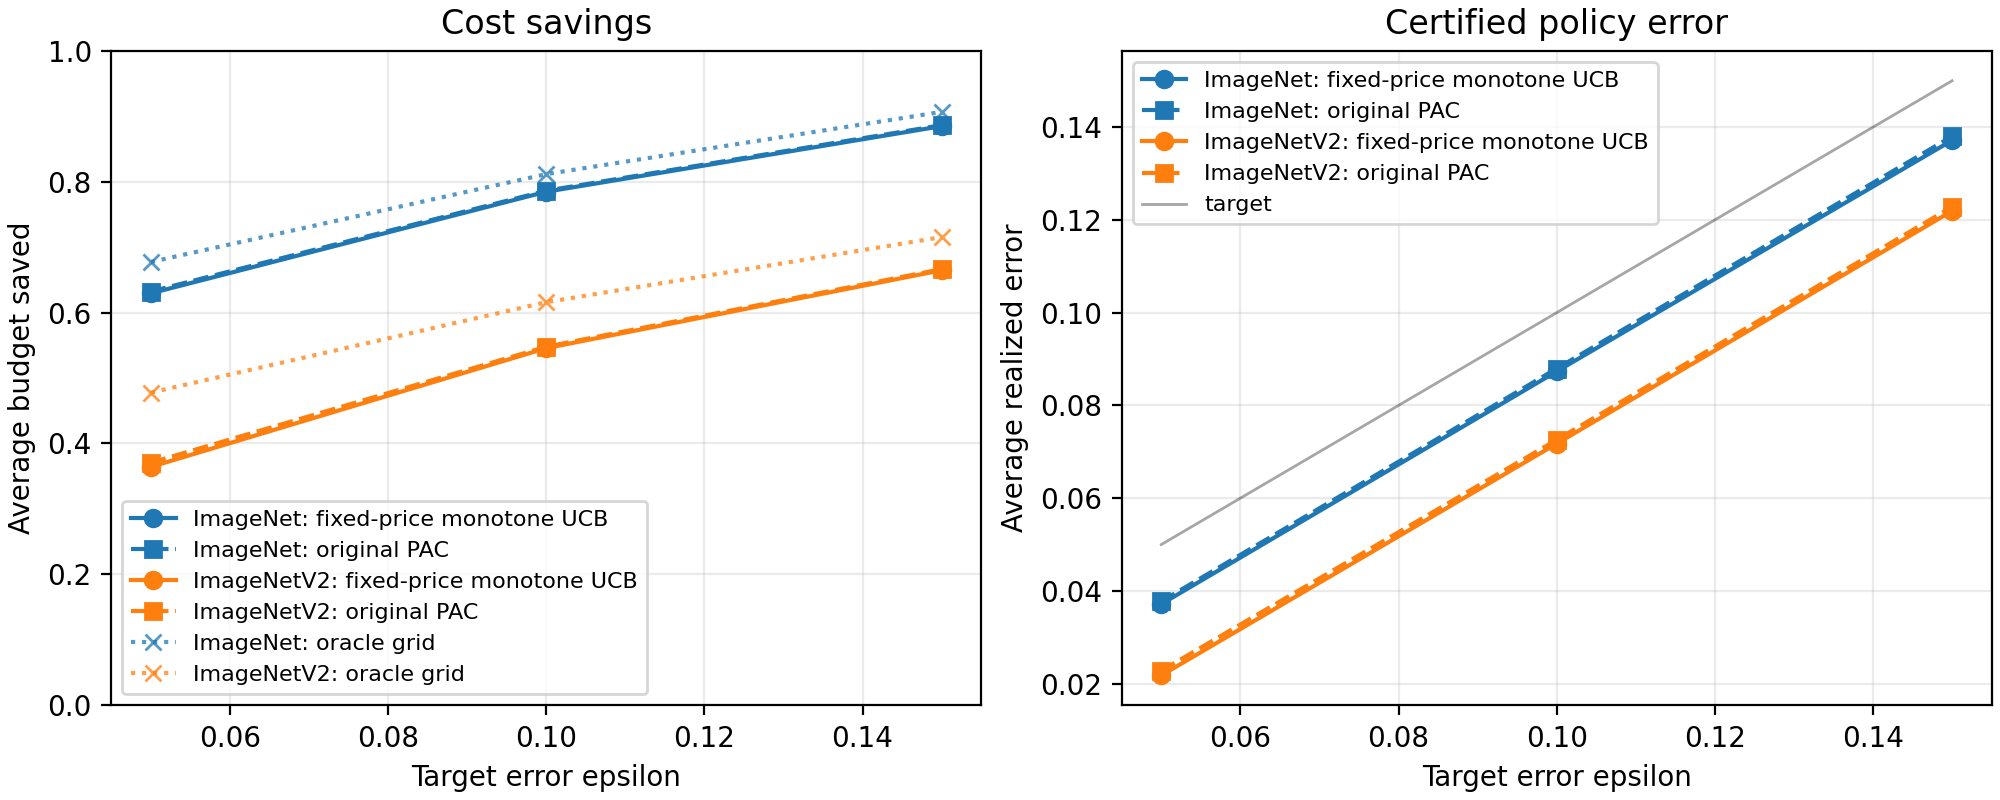
\includegraphics[width=\linewidth]{simple_offline_pac_summary.png}
      {\scriptsize One cheap source, ImageNet / ImageNetV2.}
    \end{column}
    \begin{column}{0.48\textwidth}
      \small
      \textbf{One source} ($\eps=0.10$):
      \begin{table}\centering\scriptsize
      \begin{tabular}{llcc}
        \toprule
        Data & Method & Error & Saved \\
        \midrule
        IN   & LP    & 0.087 & 0.785 \\
        IN   & PAC   & 0.088 & 0.786 \\
        INv2 & LP    & 0.072 & 0.546 \\
        INv2 & PAC   & 0.073 & 0.548 \\
        \bottomrule
      \end{tabular}
      \end{table}
      \medskip
      \begin{itemize}
        \item Error stays under target $\eps$ (0 violations).
        \item LP fixed-price $\approx$ original PAC, as predicted.
        \item Saves $\sim$78\% of expert budget on ImageNet.
      \end{itemize}
    \end{column}
  \end{columns}
\end{frame}

% ------------------------------------------------ OFFLINE EXPERIMENT 2
\begin{frame}{Offline experiments: routing beats single sources}
  \begin{columns}[T]
    \begin{column}{0.52\textwidth}
      \centering
      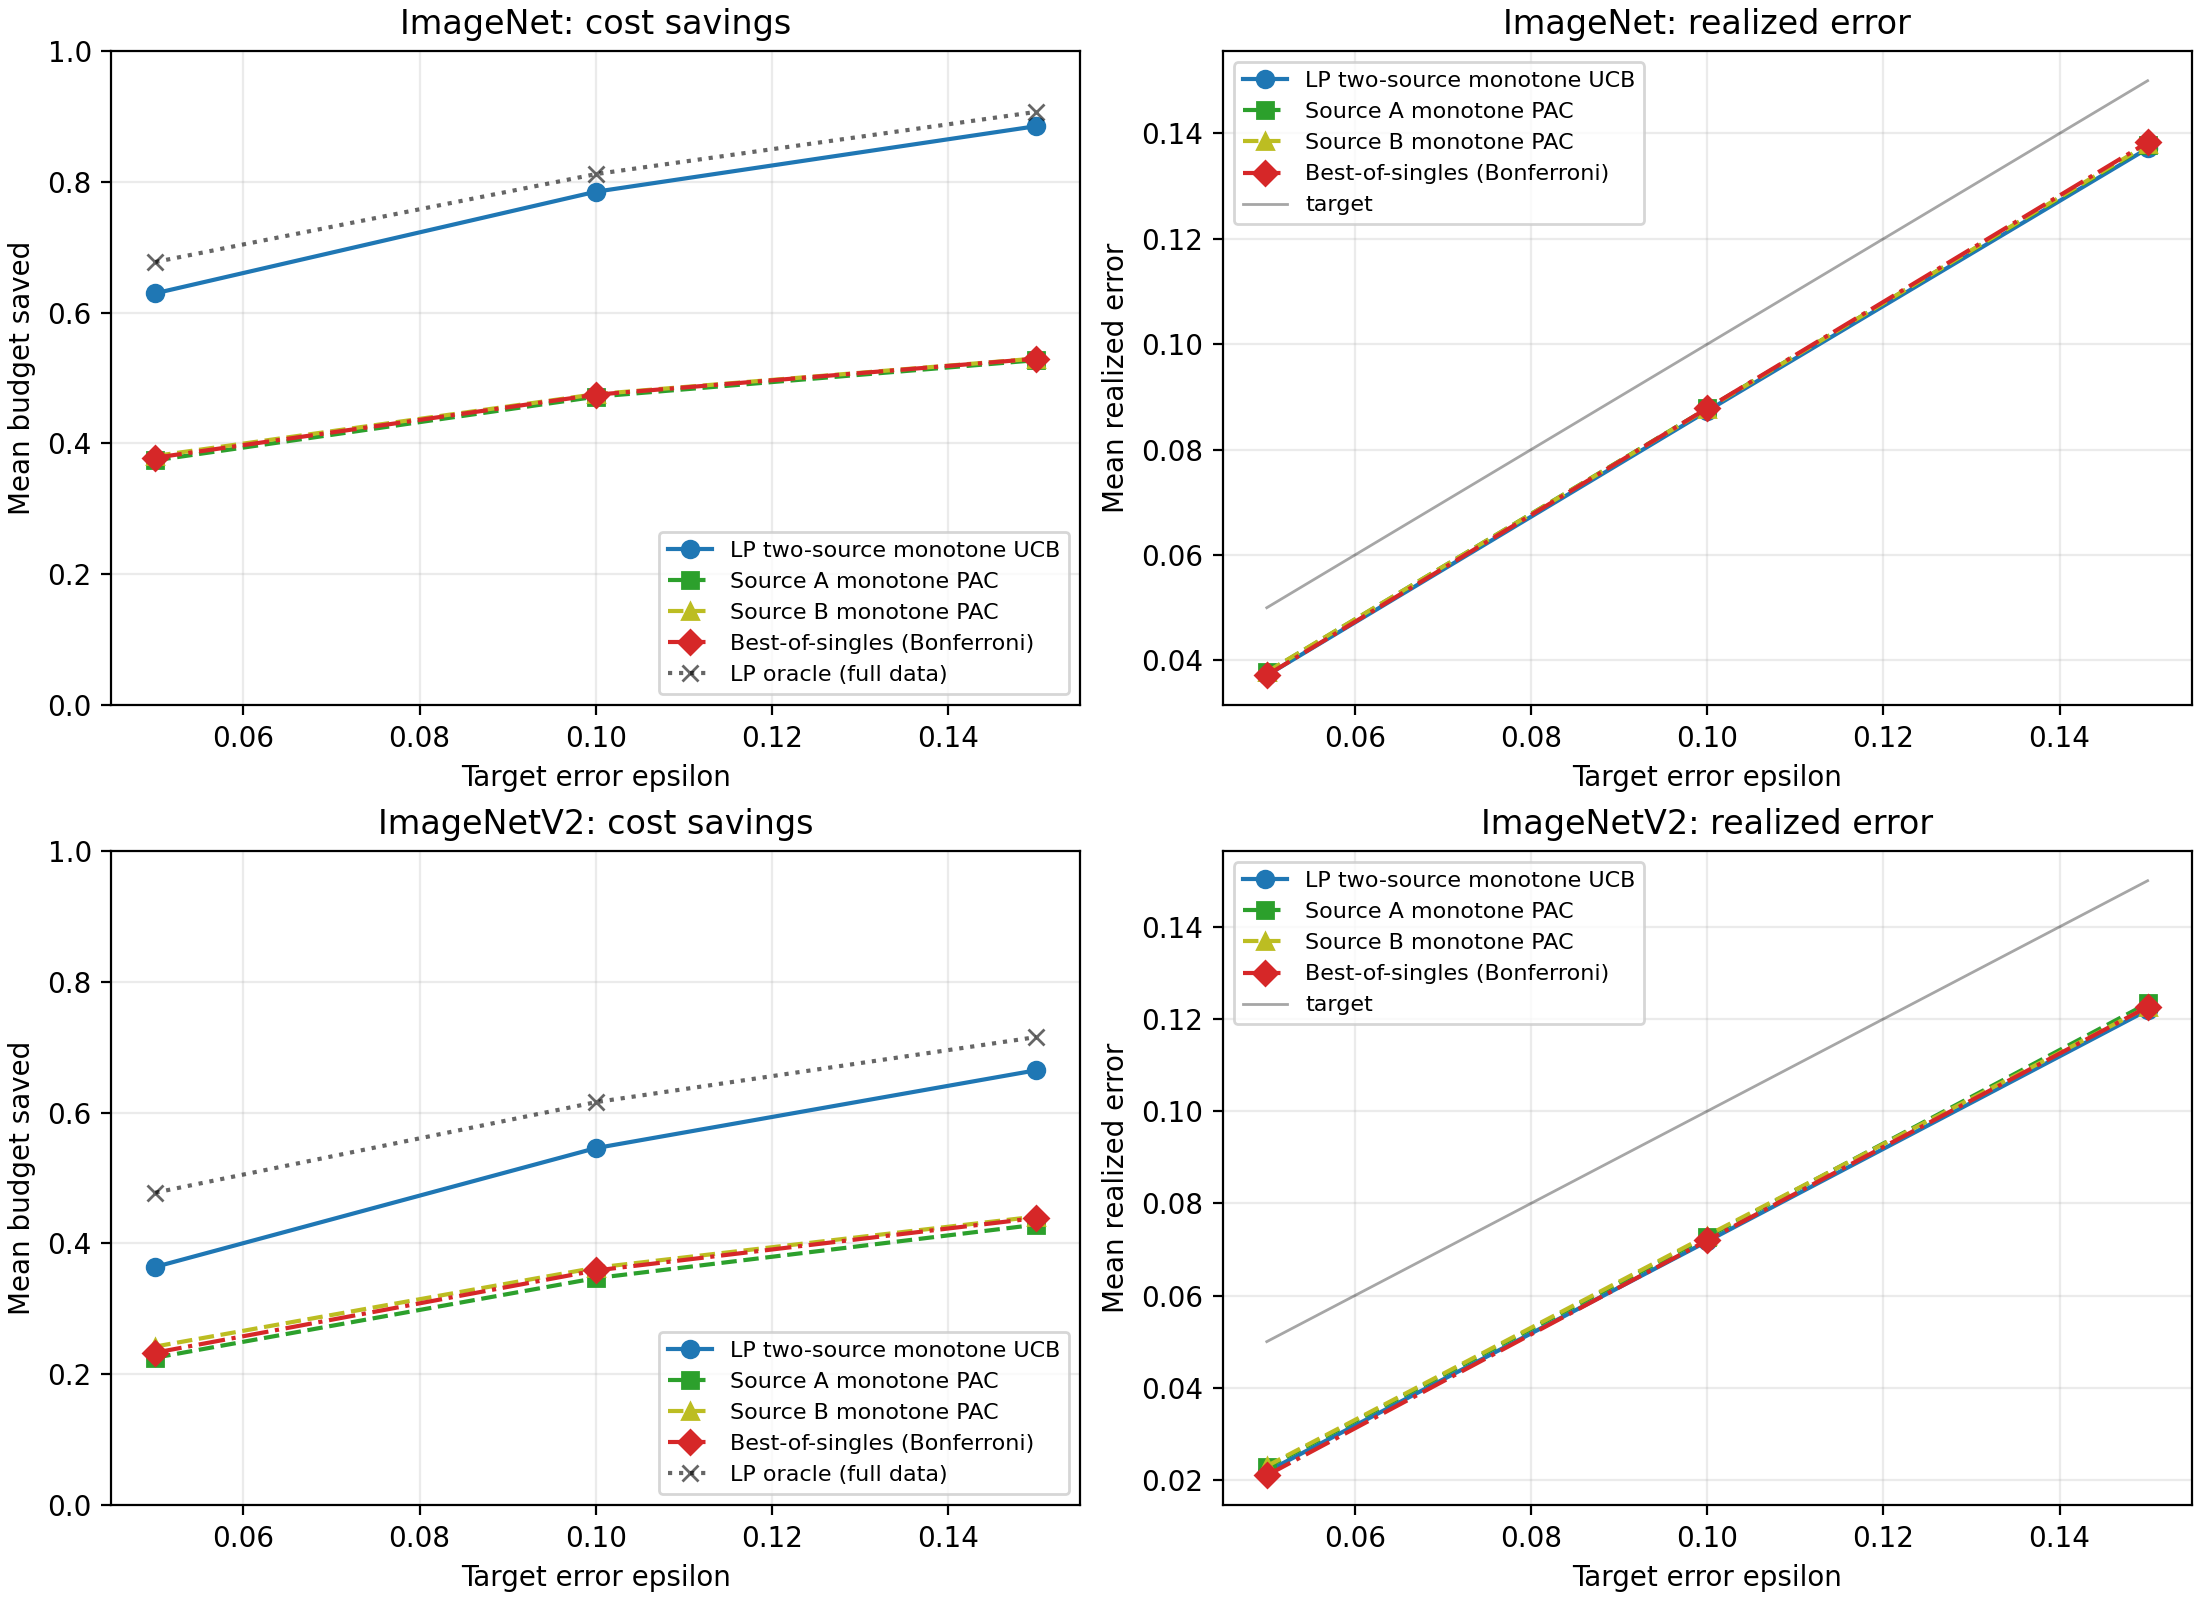
\includegraphics[width=\linewidth]{two_source_offline_pac_summary.png}
      {\scriptsize Two complementary cheap sources (by class parity).}
    \end{column}
    \begin{column}{0.48\textwidth}
      \small
      \textbf{Two sources} ($\eps=0.10$, ImageNet):
      \begin{table}\centering\scriptsize
      \begin{tabular}{lcc}
        \toprule
        Method & Error & Saved \\
        \midrule
        LP routing        & 0.087 & \textbf{0.785} \\
        Best-of-singles   & 0.088 & 0.475 \\
        \bottomrule
      \end{tabular}
      \end{table}
      \medskip
      \begin{itemize}
        \item Per-item routing to the lower-proxy source.
        \item Same error control, but \textbf{much} larger budget savings
              (0.78 vs 0.47).
        \item This is where the LP view earns its keep.
      \end{itemize}
    \end{column}
  \end{columns}
\end{frame}

% =====================================================================
\section{Online}
\begin{frame}[plain]
  \centering
  \vfill
  {\Large\bfseries\color{accent} Part II --- Online PAC Labeling via Audits}\\[6pt]
  \normalsize Items stream in; labels are hidden unless we audit.
  \vfill
\end{frame}

% ----------------------------------------------------- ONLINE SETUP
\begin{frame}{Online: a moving threshold + randomized audits}
  Items arrive one at a time. AI losses are \emph{unobserved} unless we pay the expert.
  \begin{itemize}
    \item Keep a moving price $\lambda_t$; route then threshold:
          $D_t=\ind{\hath_t^\lambda \ge 1/\lambda_t}$ (defer) .
    \item If we use the AI label, \textbf{audit} it with probability
          $p_t\in[p_{\min},1]$:
          \[
             A_t\sim\text{Bernoulli}(p_t).
          \]
          If audited, query the expert, \emph{correct} the label, and observe the AI's true error.
  \end{itemize}
  \begin{block}{Inverse-probability feedback}
    \[
       \widehat Z_t=\frac{O_t}{q_t}\,(H_t-\eps_0),
       \qquad \E[\widehat Z_t\mid \mathcal{G}_t]=H_t-\eps_0 \;\;(\text{unbiased}).
    \]
    Audited rare errors are up-weighted by $1/p_t$ to stay unbiased.
  \end{block}
\end{frame}

% ----------------------------------------------------- ONLINE UPDATE
\begin{frame}{Online: the price update}
  \[
     \lambda_{t+1}=\bigl[\lambda_t+\eta\,\widehat Z_t\bigr]_+.
  \]
  \begin{itemize}
    \item An audited \textbf{mistake} pushes $\lambda_t$ \emph{up} $\Rightarrow$
          threshold $1/\lambda_t$ drops $\Rightarrow$ routing gets more conservative.
    \item A \textbf{deferral} or a clean audit pushes $\lambda_t$ \emph{down}
          $\Rightarrow$ trust the AI more.
    \item Internal target $\eps_0\le\eps$ leaves slack for the finite-horizon bound.
  \end{itemize}
  \begin{block}{Theorem (audited online finite-horizon control)}
    With probability $\ge 1-\delta$ over audit randomness, for \emph{any} data sequence,
    \[
       \frac1T\sum_{t=1}^{T} G_t \;\le\;
       \eps_0+\frac{\Lambda_{\mathrm{on}}}{\eta T}
       +\frac{1}{p_{\min}}\sqrt{\frac{2\log(1/\delta)}{T}}.
    \]
    Choosing $\eta\asymp T^{-1/2}$ gives final error $\le\eps$, slack $O(T^{-1/2})$.
  \end{block}
\end{frame}

% -------------------------------------------------- ONLINE EXPERIMENT
\begin{frame}{Online experiments: the validity--cost knob}
  \begin{columns}[T]
    \begin{column}{0.52\textwidth}
      \centering
      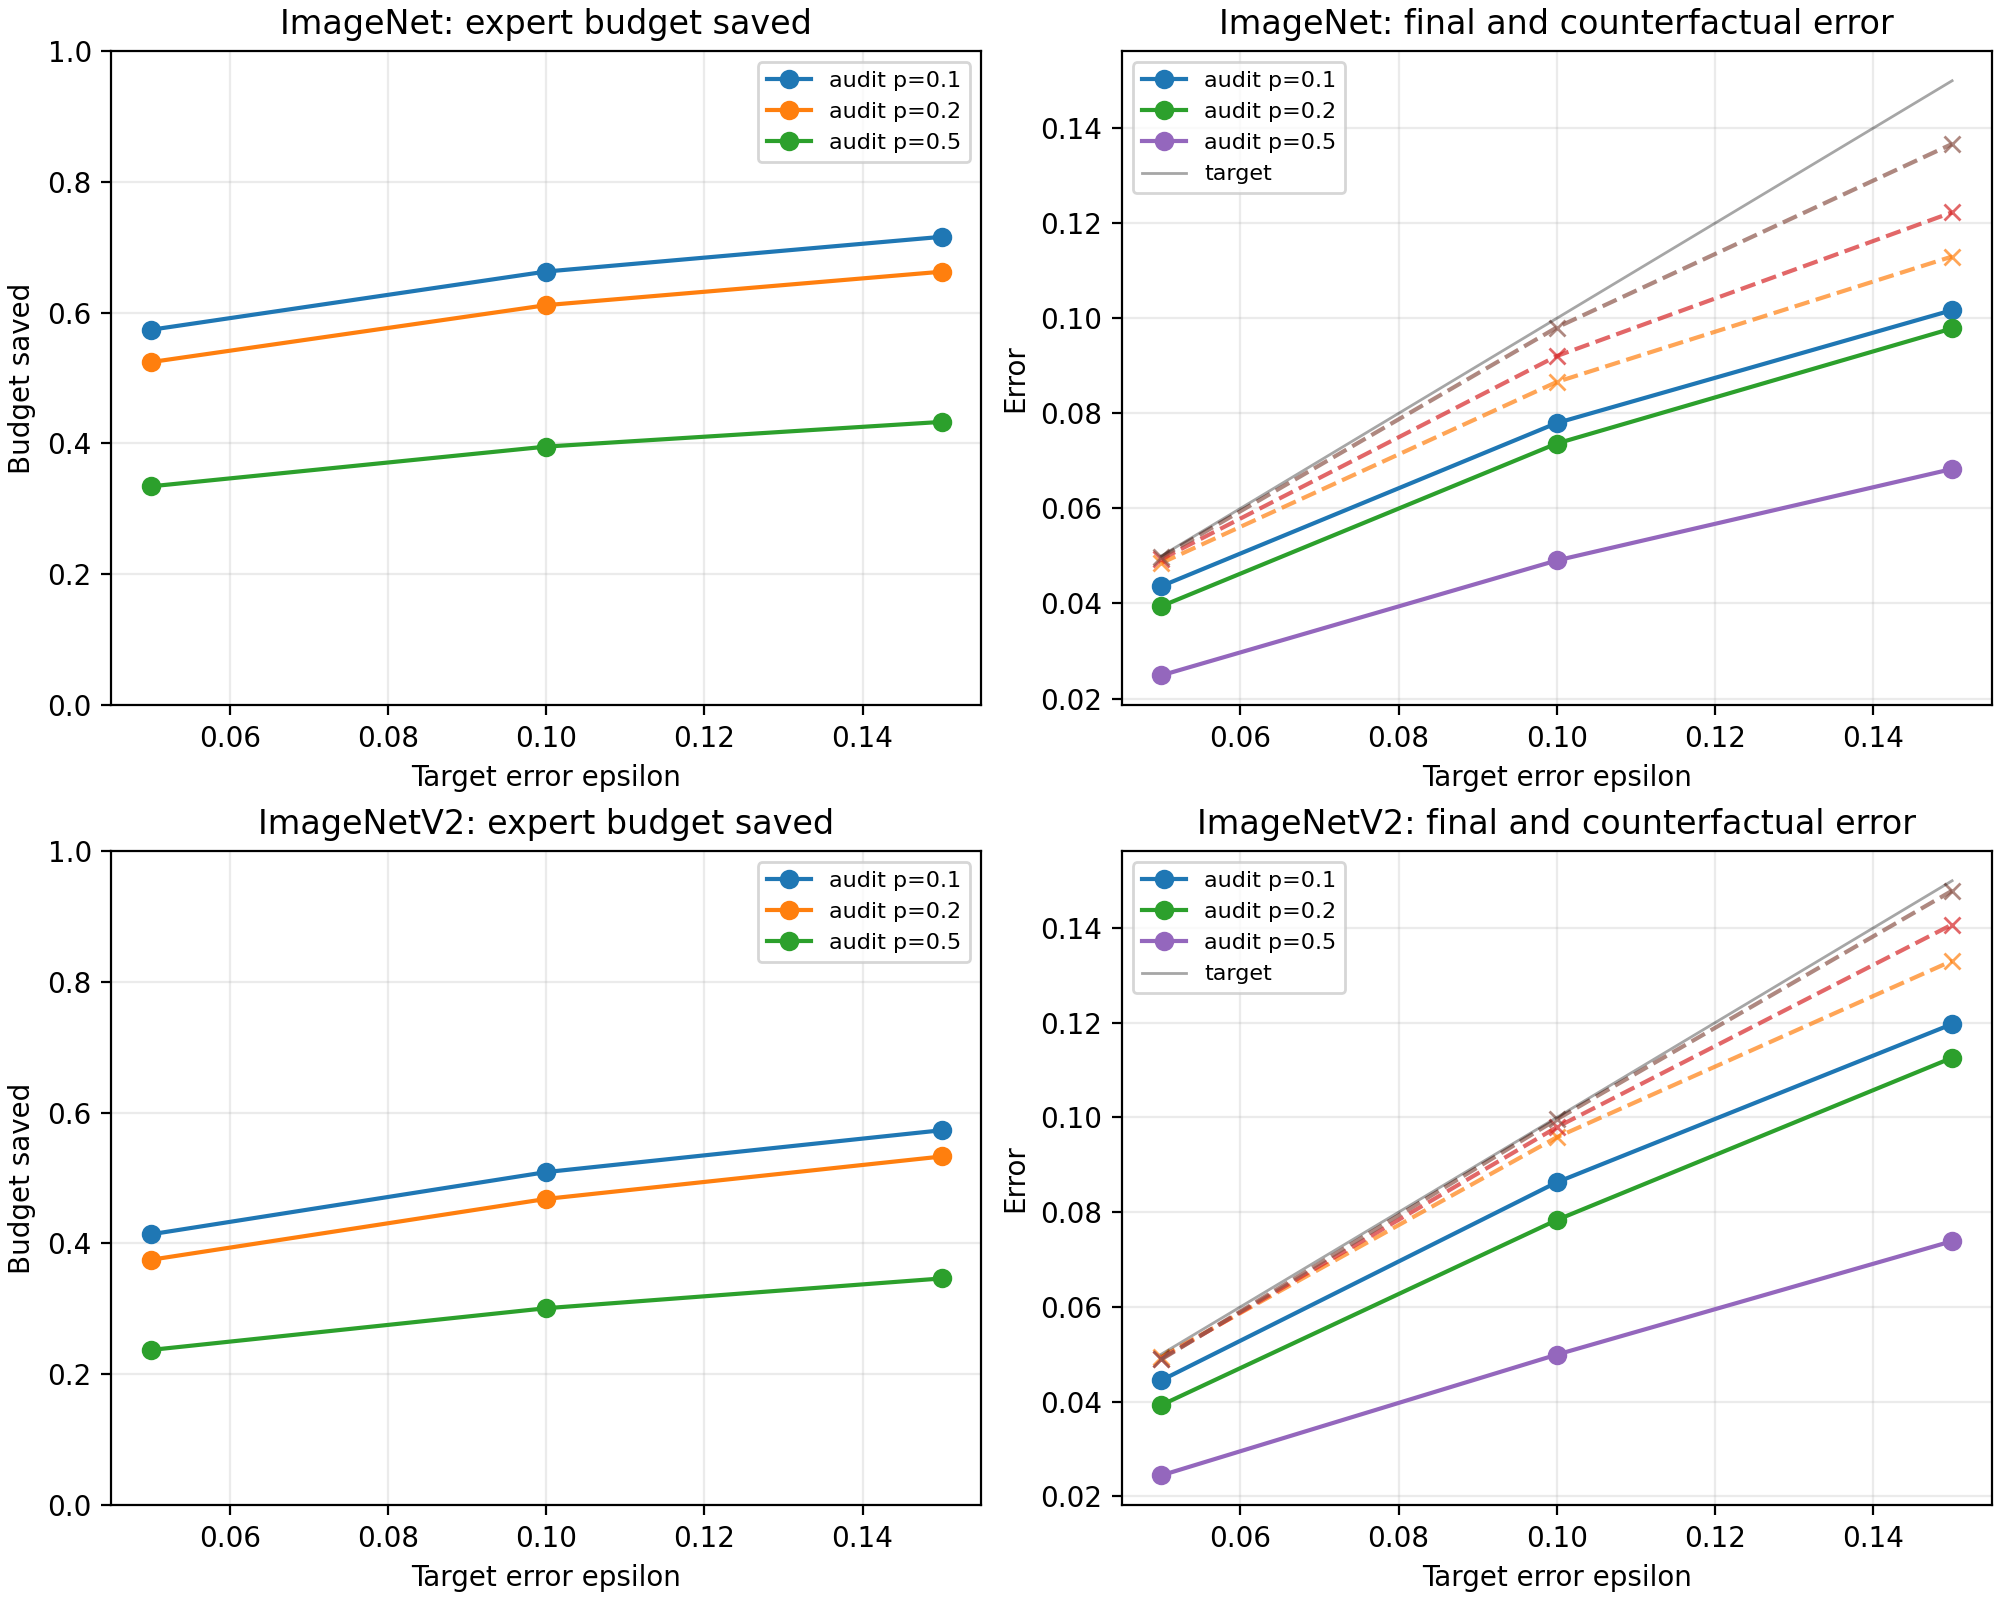
\includegraphics[width=\linewidth]{simple_online_pac_summary.png}
      {\scriptsize Audited online sweep. Dashed = AI error before correction.}
    \end{column}
    \begin{column}{0.48\textwidth}
      \small
      \textbf{Online} ($\eps=0.10$):
      \begin{table}\centering\scriptsize
      \begin{tabular}{lccc}
        \toprule
        Data & $p$ & Error & Saved \\
        \midrule
        IN   & 0.1 & 0.078 & 0.663 \\
        IN   & 0.2 & 0.074 & 0.612 \\
        IN   & 0.5 & 0.049 & 0.395 \\
        INv2 & 0.2 & 0.078 & 0.468 \\
        \bottomrule
      \end{tabular}
      \end{table}
      \medskip
      \begin{itemize}
        \item Smaller $p$: save more budget.
        \item Larger $p$: correct more, lower final error.
        \item Released-label error tracked below target under partial feedback.
      \end{itemize}
    \end{column}
  \end{columns}
\end{frame}

% --------------------------------------------------------- CONCLUSION
\begin{frame}{Takeaways}
  \begin{columns}[T]
    \begin{column}{0.5\textwidth}
      \textbf{One idea, two regimes}
      \begin{itemize}
        \item LP dual $\Rightarrow$ a single \emph{price of error} $\lambda$.
        \item \textbf{Offline:} certify $\hat\lambda$ on held-out labels.
        \item \textbf{Online:} move $\lambda_t$ with audited
              inverse-probability feedback.
      \end{itemize}
    \end{column}
    \begin{column}{0.5\textwidth}
      \textbf{What we showed}
      \begin{itemize}
        \item Proxies affect \emph{cost}, not \emph{validity}.
        \item LP rule matches PAC with one source; \emph{routing wins} with two.
        \item Online stays valid under partial feedback; $p$ trades cost vs.\ error.
      \end{itemize}
    \end{column}
  \end{columns}
  \vfill
  \begin{block}{Limitation \& next step}
    Current data has only one real cheap source. The interesting case is many
    sources with \emph{heterogeneous costs}, where a scalar threshold no longer
    suffices.
  \end{block}
  \vfill
  \centering\textbf{\color{accent}Thank you! \quad Questions?}
\end{frame}

\end{document}
